\section{Generalisation to Held-Out Instances}
\label{sec:heldout}

The result above was obtained on the grid that motivated the method, so
on its own it establishes only that the fix works where the fault was
found. Stage 2 re-runs the identical design on three instances the
modules were never tuned against, selected by the pre-specified rule of
Sec.~\ref{sec:design}. Table~\ref{tab:heldout} and
Figure~\ref{fig:heldout} give the outcome; all four grids completed
144/144 trials.

\textbf{The canonical effect replicates.} On $(N{=}21,a{=}2,r{=}6)$ ---
same order, base never used in design --- Full raised success from 50.0\%
to 97.9\%, $+47.9$ percentage points ($b{=}0$, $c{=}69$,
$p=3.4\times10^{-21}$), numerically the same gain as on the canonical
instance; B and D reproduce their canonical effects ($+26.4$ and
$+29.2$ pp) and B again beats C ($+21.5$ pp, $p=3.1\times10^{-6}$). This
is the paper's generalisation evidence, and it is why the circularity
objection does not stand. It also lands at \textbf{97.9\%, not 100\%}:
three of 144 trials still fail, so the honest summary of the method's
ceiling on instances with headroom is $97.9$--$100\%$.

\textbf{Where the baseline has no headroom, no module helps or hurts.} On
$(N{=}21,a{=}8,r{=}2)$ the published pipeline already succeeds on every
trial and every arm returns 100\% with zero discordant pairs --- a ceiling
effect, not a null effect. That instance is also the clearest in-corpus
demonstration of the small-order confound: at order two the
continued-fraction stage recovers the order from almost any phase, so
nothing upstream can be observed to matter. On $(N{=}15,a{=}2,r{=}4)$
baseline succeeds 88.9\% of the time, and B and Full close the gap
completely ($+11.1$ pp, $b{=}0$, $c{=}16$, $p=3.1\times10^{-5}$) while C
changes nothing and D nets exactly zero, fixing eight trials and breaking
eight.

\textbf{The two weaker modules show their weakness here.} Module C is
null on two of three held-out instances, and on the third repeats the
marginal $+4.9$ pp that fails Holm correction (\SItables{}).
Module D carries the most two-sided discordant counts anywhere in the
study --- $(6,41)$ canonical, $(8,50)$ on the replication, $(8,8)$ on
$(N{=}15,a{=}2)$ --- because additional shots change which pattern ranks
first, and a changed ranking sometimes sends continued-fraction recovery
down an unsuccessful branch. D's aggregate effect is strongly positive
where headroom exists, but its per-trial variance is real.

\begin{table}[htbp]
\centering\small
\caption{Held-out generalisation: baseline versus the full combination on
all four instances, 144 seed-paired trials each. The three held-out
instances were selected by a rule fixed before any trial of that stage
ran. $b$ = trials the arm broke; $c$ = trials it fixed; $p$ is the exact
two-sided binomial McNemar value, uncorrected (these are replications,
not members of the Holm family, \SItables{}). Per-arm rows for
B, C and D on every instance are in \SItables{}, and are plotted in
Fig.~\ref{fig:heldout}.}
\label{tab:heldout}
\resizebox{\linewidth}{!}{%
\begin{tabular}{@{}lccccc@{}}
\toprule
Instance & Baseline & Full & Diff.\ [95\% CI] & $(b,c)$ & Exact $p$ \\
\midrule
$N{=}21$, $a{=}19$, $r{=}6$ \emph{(canonical)}
 & 52.1\% & \textbf{100.0\%} & $+47.9$ pp $[+39.6,+56.3]$ & $(0,69)$ & $3.4\times10^{-21}$ \\
$N{=}21$, $a{=}2$, $r{=}6$ \emph{(held-out)}
 & 50.0\% & \textbf{97.9\%}  & $+47.9$ pp $[+39.6,+56.3]$ & $(0,69)$ & $3.4\times10^{-21}$ \\
$N{=}15$, $a{=}2$, $r{=}4$ \emph{(held-out)}
 & 88.9\% & \textbf{100.0\%} & $+11.1$ pp $[+6.3,+16.0]$  & $(0,16)$ & $3.1\times10^{-5}$ \\
$N{=}21$, $a{=}8$, $r{=}2$ \emph{(held-out, ceiling)}
 & 100.0\% & 100.0\% & $\phantom{0}+0.0$ pp $[+0.0,+0.0]$ & $(0,0)$ & $1.00$ \\
\bottomrule
\end{tabular}
}
\end{table}

\begin{figure}[htbp]
\centering
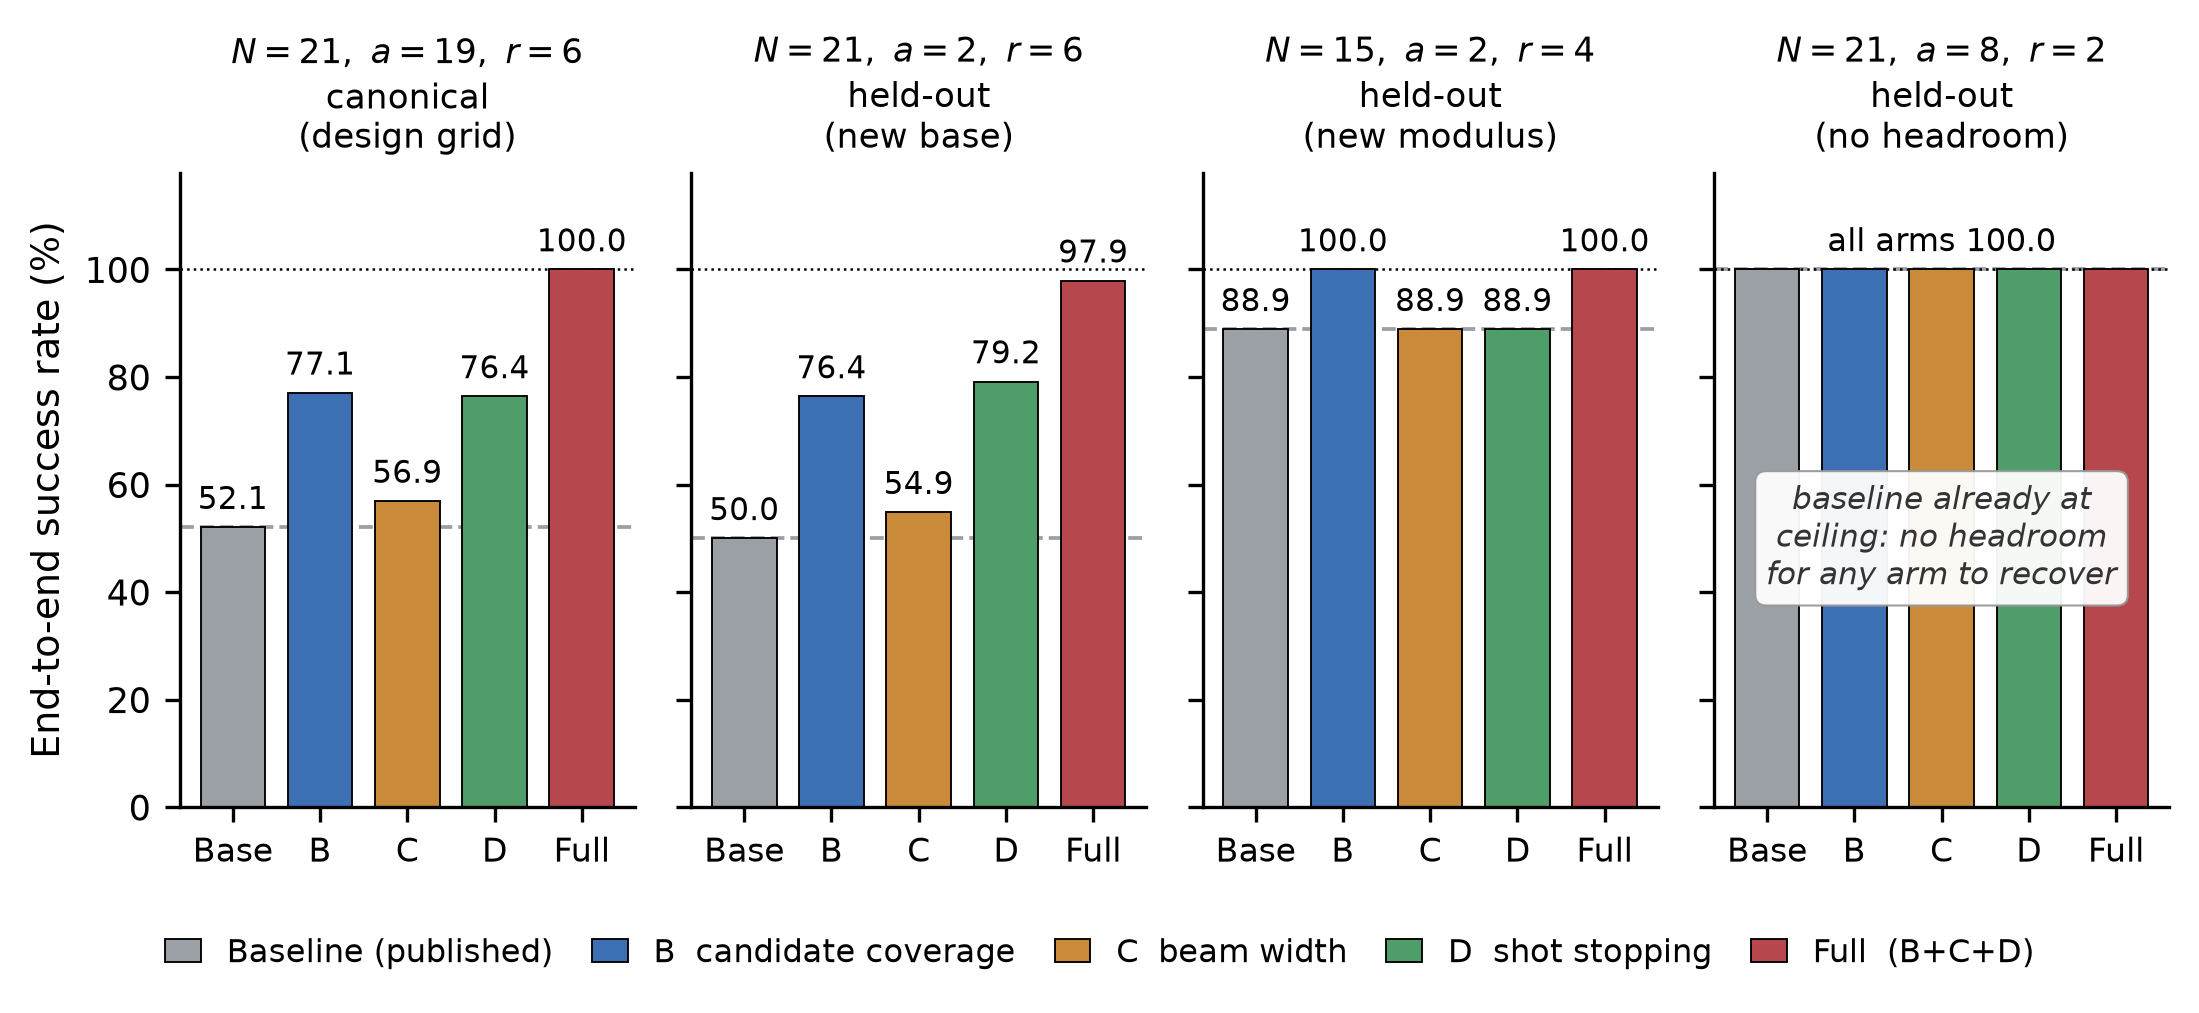
\includegraphics[width=0.94\linewidth]{../Data/failure_study/plots/paper_fig3_heldout.png}
\caption{\textbf{Does the canonical result survive on instances the
modules were never tuned against?} Per-arm end-to-end success on the
canonical instance (left) and the three pre-specified held-out
instances, 144 seed-paired trials each. Dashed line: that panel's
baseline. Dotted line: the 100\% ceiling. The canonical effect replicates
on $(N{=}21,a{=}2,r{=}6)$, a base never used in design, at 97.9\% rather
than 100\%. Headroom shrinks left to right: on $(N{=}15,a{=}2,r{=}4)$
only B and Full move the result, and on $(N{=}21,a{=}8,r{=}2)$ the
published pipeline already succeeds on every trial, so no arm can
demonstrate anything --- a ceiling effect, not a null effect. Module C
changes nothing on either right-hand instance. Rendered from
\texttt{phase6\_ablation\_diagnostics.csv} and
\texttt{phase7\_heldout\_*.csv}.}
\label{fig:heldout}
\end{figure}
